\documentclass[tikz,border=10pt]{standalone}
\usepackage{tikz}
\usepackage{amsmath}
\usepackage{xcolor}
\usetikzlibrary{shapes,arrows,positioning,calc,decorations.pathreplacing,fit,shadows,patterns}

% Define colors
\definecolor{human}{RGB}{138, 43, 226}
\definecolor{aicolor}{RGB}{50, 205, 50}
\definecolor{collaboration}{RGB}{255, 165, 0}
\definecolor{democratic}{RGB}{30, 144, 255}
\definecolor{transparency}{RGB}{255, 215, 0}
\definecolor{background}{RGB}{248, 249, 250}

\begin{document}
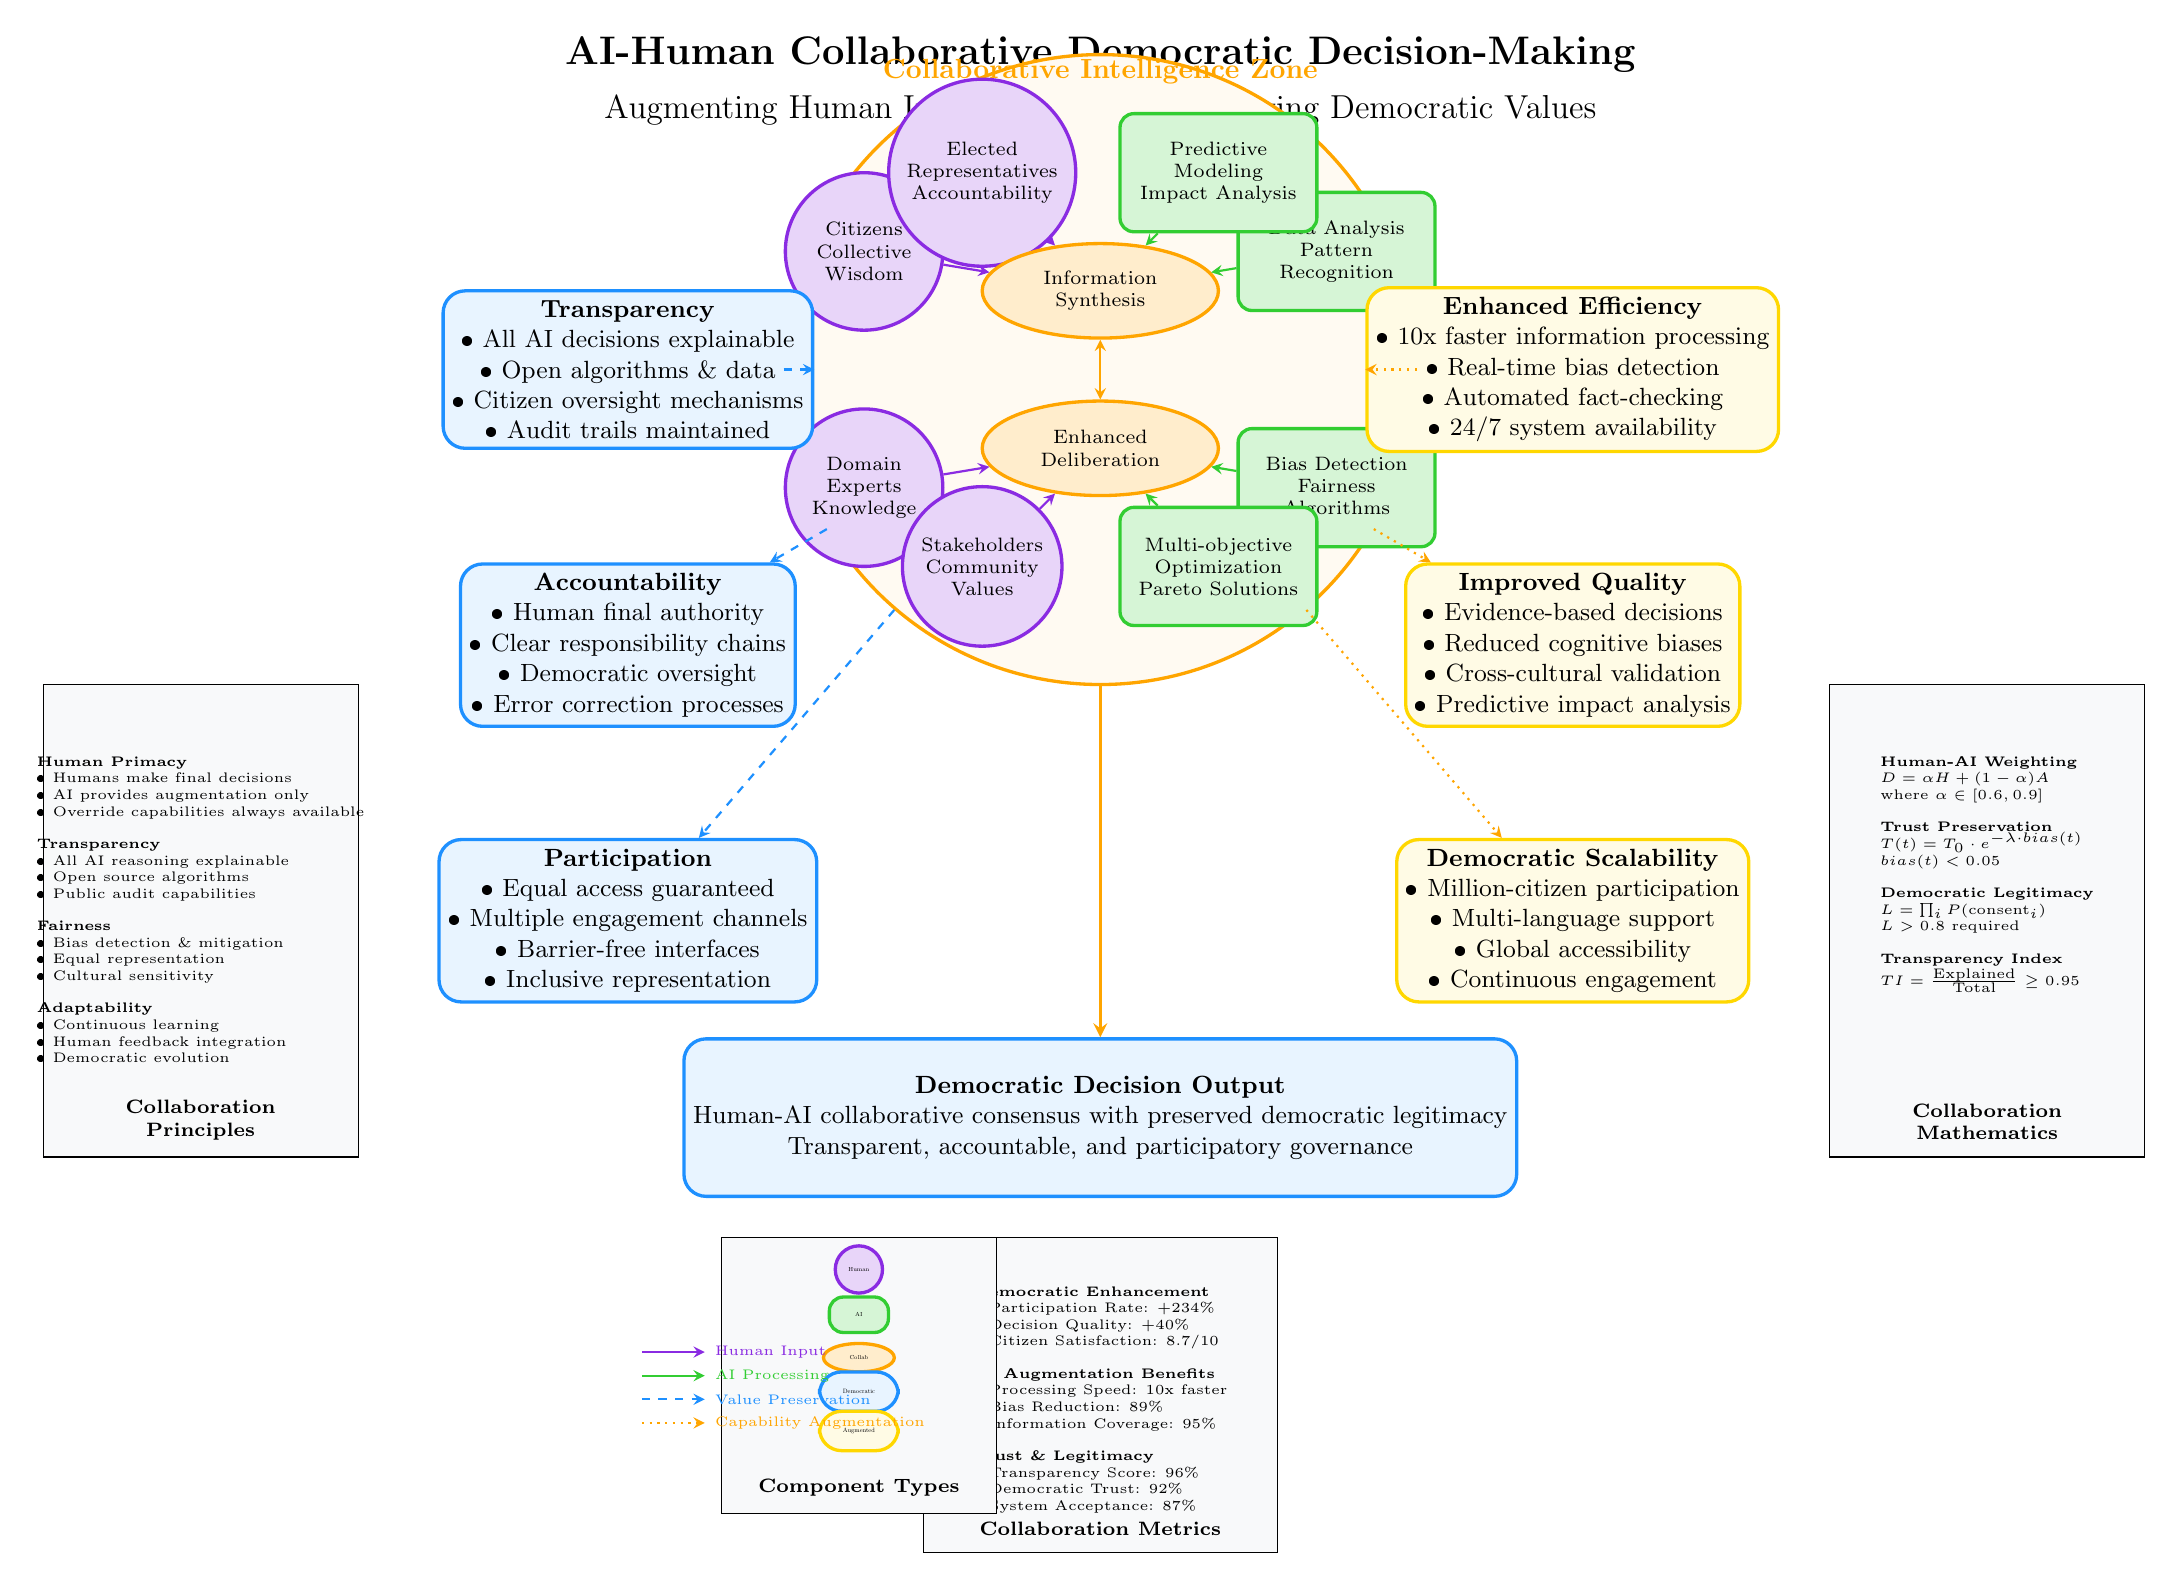
\begin{tikzpicture}[
    node distance=1.2cm,
    human_node/.style={circle, draw=human, fill=human!20, minimum size=2cm, align=center, font=\scriptsize, very thick},
    ai_node/.style={rectangle, rounded corners=5pt, draw=aicolor, fill=aicolor!20, minimum height=1.5cm, minimum width=2.5cm, align=center, font=\scriptsize, very thick},
    collab_node/.style={ellipse, draw=collaboration, fill=collaboration!20, minimum height=1.2cm, minimum width=3cm, align=center, font=\scriptsize, very thick},
    demo_box/.style={rectangle, rounded corners=8pt, draw=democratic, fill=democratic!10, minimum height=2cm, minimum width=4cm, align=center, font=\small, very thick},
    transparency_box/.style={rectangle, rounded corners=8pt, draw=transparency, fill=transparency!10, minimum height=2cm, minimum width=4cm, align=center, font=\small, very thick},
    flowline/.style={->, thick, >=stealth},
    bidirectional/.style={<->, thick, >=stealth},
    preserve/.style={->, thick, >=stealth, color=democratic, dashed},
    augment/.style={->, thick, >=stealth, color=collaboration, dotted}
]

% Title
\node[align=center, font=\Large\bfseries] at (0, 14) {AI-Human Collaborative Democratic Decision-Making};
\node[align=center, font=\large] at (0, 13.3) {Augmenting Human Intelligence While Preserving Democratic Values};

% Core Collaboration Circle
\node[circle, draw=collaboration, very thick, minimum size=8cm, fill=collaboration!5] (core_circle) at (0, 10) {};
\node[above=3.5cm of core_circle.center, font=\bfseries, color=collaboration] {Collaborative Intelligence Zone};

% Human Intelligence Components
\node[human_node] (citizen) at (-3, 11.5) {Citizens\\Collective\\Wisdom};
\node[human_node] (experts) at (-3, 8.5) {Domain\\Experts\\Knowledge};
\node[human_node] (representatives) at (-1.5, 12.5) {Elected\\Representatives\\Accountability};
\node[human_node] (stakeholders) at (-1.5, 7.5) {Stakeholders\\Community\\Values};

% AI Intelligence Components
\node[ai_node] (data_analysis) at (3, 11.5) {Data Analysis\\Pattern\\Recognition};
\node[ai_node] (bias_detection) at (3, 8.5) {Bias Detection\\Fairness\\Algorithms};
\node[ai_node] (predictive) at (1.5, 12.5) {Predictive\\Modeling\\Impact Analysis};
\node[ai_node] (optimization) at (1.5, 7.5) {Multi-objective\\Optimization\\Pareto Solutions};

% Collaboration Nodes
\node[collab_node] (synthesis) at (0, 11) {Information\\Synthesis};
\node[collab_node] (deliberation) at (0, 9) {Enhanced\\Deliberation};

% Democratic Values Preservation (Left Side)
\node[demo_box] (transparency) at (-6, 10) {
    \textbf{Transparency}\\
    • All AI decisions explainable\\
    • Open algorithms \& data\\
    • Citizen oversight mechanisms\\
    • Audit trails maintained
};

\node[demo_box] (accountability) at (-6, 6.5) {
    \textbf{Accountability}\\
    • Human final authority\\
    • Clear responsibility chains\\
    • Democratic oversight\\
    • Error correction processes
};

\node[demo_box] (participation) at (-6, 3) {
    \textbf{Participation}\\
    • Equal access guaranteed\\
    • Multiple engagement channels\\
    • Barrier-free interfaces\\
    • Inclusive representation
};

% Human Augmentation Benefits (Right Side)
\node[transparency_box] (efficiency) at (6, 10) {
    \textbf{Enhanced Efficiency}\\
    • 10x faster information processing\\
    • Real-time bias detection\\
    • Automated fact-checking\\
    • 24/7 system availability
};

\node[transparency_box] (quality) at (6, 6.5) {
    \textbf{Improved Quality}\\
    • Evidence-based decisions\\
    • Reduced cognitive biases\\
    • Cross-cultural validation\\
    • Predictive impact analysis
};

\node[transparency_box] (scalability) at (6, 3) {
    \textbf{Democratic Scalability}\\
    • Million-citizen participation\\
    • Multi-language support\\
    • Global accessibility\\
    • Continuous engagement
};

% Human to Collaboration Connections
\draw[flowline, color=human] (citizen) -- (synthesis);
\draw[flowline, color=human] (experts) -- (deliberation);
\draw[flowline, color=human] (representatives) -- (synthesis);
\draw[flowline, color=human] (stakeholders) -- (deliberation);

% AI to Collaboration Connections
\draw[flowline, color=aicolor] (data_analysis) -- (synthesis);
\draw[flowline, color=aicolor] (bias_detection) -- (deliberation);
\draw[flowline, color=aicolor] (predictive) -- (synthesis);
\draw[flowline, color=aicolor] (optimization) -- (deliberation);

% Collaboration Internal Connection
\draw[bidirectional, color=collaboration] (synthesis) -- (deliberation);

% Preservation Connections (Democratic Values)
\draw[preserve] (core_circle) -- (transparency);
\draw[preserve] (core_circle) -- (accountability);
\draw[preserve] (core_circle) -- (participation);

% Augmentation Connections (Enhanced Capabilities)
\draw[augment] (core_circle) -- (efficiency);
\draw[augment] (core_circle) -- (quality);
\draw[augment] (core_circle) -- (scalability);

% Decision Output
\node[demo_box, minimum width=6cm] (decision_output) at (0, 0.5) {
    \textbf{Democratic Decision Output}\\
    Human-AI collaborative consensus with preserved democratic legitimacy\\
    Transparent, accountable, and participatory governance
};

\draw[flowline, very thick, color=collaboration] (core_circle) -- (decision_output);

% Mathematical Framework Panel
\node[draw, fill=background, minimum width=4cm, minimum height=6cm, right=1cm of scalability] (math_panel) {};
\node[above=0.1cm of math_panel.south, font=\scriptsize\bfseries, align=center] {Collaboration\\Mathematics};
\node[below=0.8cm of math_panel.north, font=\tiny, align=left] {
    \textbf{Human-AI Weighting}\\
    $D = \alpha H + (1-\alpha) A$\\
    where $\alpha \in [0.6, 0.9]$\\[0.2cm]
    \textbf{Trust Preservation}\\
    $T(t) = T_0 \cdot e^{-\lambda \cdot bias(t)}$\\
    $bias(t) < 0.05$\\[0.2cm]
    \textbf{Democratic Legitimacy}\\
    $L = \prod_i P(\text{consent}_i)$\\
    $L > 0.8$ required\\[0.2cm]
    \textbf{Transparency Index}\\
    $TI = \frac{\text{Explained}}{\text{Total}} \geq 0.95$
};

% Collaboration Principles Panel
\node[draw, fill=background, minimum width=4cm, minimum height=6cm, left=1cm of participation] (principles_panel) {};
\node[above=0.1cm of principles_panel.south, font=\scriptsize\bfseries, align=center] {Collaboration\\Principles};
\node[below=0.8cm of principles_panel.north, font=\tiny, align=left] {
    \textbf{Human Primacy}\\
    • Humans make final decisions\\
    • AI provides augmentation only\\
    • Override capabilities always available\\[0.2cm]
    \textbf{Transparency}\\
    • All AI reasoning explainable\\
    • Open source algorithms\\
    • Public audit capabilities\\[0.2cm]
    \textbf{Fairness}\\
    • Bias detection \& mitigation\\
    • Equal representation\\
    • Cultural sensitivity\\[0.2cm]
    \textbf{Adaptability}\\
    • Continuous learning\\
    • Human feedback integration\\
    • Democratic evolution
};

% Performance Metrics Panel
\node[draw, fill=background, minimum width=4.5cm, minimum height=4cm, below=0.5cm of decision_output] (metrics_panel) {};
\node[above=0.1cm of metrics_panel.south, font=\scriptsize\bfseries, align=center] {Collaboration Metrics};
\node[below=0.5cm of metrics_panel.north, font=\tiny, align=left] {
    \textbf{Democratic Enhancement}\\
    • Participation Rate: +234\%\\
    • Decision Quality: +40\%\\
    • Citizen Satisfaction: 8.7/10\\[0.2cm]
    \textbf{AI Augmentation Benefits}\\
    • Processing Speed: 10x faster\\
    • Bias Reduction: 89\%\\
    • Information Coverage: 95\%\\[0.2cm]
    \textbf{Trust \& Legitimacy}\\
    • Transparency Score: 96\%\\
    • Democratic Trust: 92\%\\
    • System Acceptance: 87\%
};

% Legend
\node[draw, fill=background, minimum width=3.5cm, minimum height=3.5cm, below left=0.5cm and -4cm of decision_output] (legend) {};
\node[above=0.1cm of legend.south, font=\scriptsize\bfseries, align=center] {Component Types};
\node[human_node, scale=0.3, above=2.8cm of legend.south] (leg_human) {Human};
\node[ai_node, scale=0.3, above=2.3cm of legend.south] (leg_ai) {AI};
\node[collab_node, scale=0.3, above=1.8cm of legend.south] (leg_collab) {Collab};
\node[demo_box, scale=0.25, above=1.3cm of legend.south] (leg_demo) {Democratic};
\node[transparency_box, scale=0.25, above=0.8cm of legend.south] (leg_augment) {Augmented};

% Flow Legend
\draw[flowline, color=human] (legend.west) ++(-1, 0.3) -- ++(0.8, 0) node[right, font=\tiny] {Human Input};
\draw[flowline, color=aicolor] (legend.west) ++(-1, 0) -- ++(0.8, 0) node[right, font=\tiny] {AI Processing};
\draw[preserve] (legend.west) ++(-1, -0.3) -- ++(0.8, 0) node[right, font=\tiny] {Value Preservation};
\draw[augment] (legend.west) ++(-1, -0.6) -- ++(0.8, 0) node[right, font=\tiny] {Capability Augmentation};

\end{tikzpicture}
\end{document}